\documentclass[conference]{IEEEtran}

\usepackage{cite}
\usepackage{amsmath,amssymb}
\usepackage{graphicx}
\usepackage{booktabs}
\usepackage{url}
\usepackage{tikz}
\usetikzlibrary{arrows.meta}

\begin{document}

\title{Kimi K2: Architecture of a Trillion-Parameter\\Mixture-of-Experts Language Model}

\author{\IEEEauthorblockN{Nagham Taweel}
\IEEEauthorblockA{NLP \& AI Internship, Cellula Technologies\\
naghamatawel@gmail.com}}

\maketitle

\begin{abstract}
Kimi K2 is an open-weight large language model developed by Moonshot AI and optimized for agentic tasks such as tool use, coding, and multi-step problem solving. Kimi K2 is a Mixture-of-Experts (MoE) Transformer with 1.04 trillion total and 32 billion activated parameters, built from 384 routed experts, of which eight are selected per token, plus one shared expert. It uses Multi-head Latent Attention (MLA) with 64 heads, half as many as DeepSeek-V3, to reduce long-context inference cost. The model was pre-trained on 15.5 trillion tokens with MuonClip, an optimizer that combines Muon with a per-head QK-Clip mechanism and removed loss spikes at trillion-parameter scale. We explain the key equations and compare the design with DeepSeek-V3. Kimi K2's main contributions lie in higher sparsity, cheaper attention, stable optimization, and agentic post-training rather than in a new layer type.
\end{abstract}

\begin{IEEEkeywords}
Kimi K2, large language models, mixture of experts, multi-head latent attention, MuonClip, agentic intelligence
\end{IEEEkeywords}

\section{Introduction}
Large language models (LLMs) are moving from passive chat assistants toward \emph{agentic intelligence}, defined by the Kimi team as ``the capabilities for models to autonomously perceive, plan, reason, and act within complex and dynamic environments''~\cite{kimik2}. Kimi K2, released by Moonshot AI with its technical report in July 2025, is an open-weight model designed for this setting~\cite{kimik2,kimik2github}. It is a 1.04-trillion-parameter MoE Transformer that activates only 32B parameters per token~\cite{kimik2}, and both its code and weights are published under a modified MIT license~\cite{kimik2github}.

The family includes Kimi-K2-Base, a foundation model intended for fine-tuning, and Kimi-K2-Instruct, a post-trained ``reflex-grade model without long thinking'' for chat and agentic use~\cite{kimik2github}. Later releases include Kimi-K2-Instruct-0905, which extends the context window from 128K to 256K tokens, and Kimi K2 Thinking, which reasons step by step while calling tools~\cite{kimik2thinking}. Its intended applications are tool use, reasoning, coding, and autonomous problem solving~\cite{kimik2github}; this paper focuses on the architecture in the technical report.

Architecturally, K2 follows DeepSeek-V3~\cite{deepseekv3}: it combines a highly sparse MoE feed-forward layer with MLA~\cite{deepseekv2}. The report lists three main contributions: the MuonClip optimizer, a large-scale agentic data synthesis pipeline, and a reinforcement learning (RL) framework that combines verifiable rewards with self-critique rubric rewards~\cite{kimik2}.

\section{Mixture-of-Experts Architecture}
An MoE layer replaces the single feed-forward network (FFN) of a Transformer block with many smaller FFNs, called experts, and a router that sends each token to only a few of them~\cite{shazeer2017}. Model capacity therefore grows with the total number of experts, while the computation per token depends only on the experts that are selected.

\textbf{Organization.} Kimi K2 has 61 layers. The first layer uses a dense FFN, and the other 60 use MoE layers~\cite{kimik2}. Each MoE layer contains 384 routed experts and one shared expert. Each expert is a SwiGLU FFN with a hidden dimension of 2048, and the model hidden dimension is 7168~\cite{kimik2,kimik2github}. For every token, eight routed experts are selected and the shared expert is always applied.

\textbf{Routing.} The K2 report states that the architecture is similar to DeepSeek-V3 but does not restate the routing equations, so we use the DeepSeekMoE formulation of~\cite{deepseekv3}. For the input $\mathbf{u}_t$ of token $t$, the layer output is
\begin{equation}
\mathbf{h}'_t=\mathbf{u}_t+\mathrm{FFN}^{(s)}(\mathbf{u}_t)+\sum_{i=1}^{N_r} g_{i,t}\,\mathrm{FFN}^{(r)}_i(\mathbf{u}_t),
\end{equation}
where $\mathrm{FFN}^{(s)}$ is the shared expert, $N_r=384$ is the number of routed experts, and $g_{i,t}$ is the gate of expert $i$. The gates are computed from token-to-expert affinities:
\begin{align}
s_{i,t}&=\sigma\!\left(\mathbf{u}_t^{\top}\mathbf{e}_i\right),\\
g'_{i,t}&=s_{i,t}\cdot\mathbf{1}\!\left[s_{i,t}+b_i\in\mathrm{Top}K\{s_{j,t}+b_j\}\right],\\
g_{i,t}&=g'_{i,t}\Big/\textstyle\sum_{j=1}^{N_r} g'_{j,t},
\end{align}
where $\mathbf{e}_i$ is a learned centroid of expert $i$, $\sigma$ is the sigmoid function, and $K=8$. The bias $b_i$ affects only \emph{which} experts are selected, not the gate values. After each training step it is decreased for overloaded experts and increased for underloaded ones. This balances the load without a large auxiliary loss~\cite{deepseekv3}. The selected experts' outputs are weighted by the normalized gates and added to the shared expert's output and the residual connection (Fig.~\ref{fig:arch}).

\textbf{Sparsity.} The report defines sparsity as the ratio of total to activated experts. K2 uses $384/8=48$, compared with $256/8=32$ in DeepSeek-V3~\cite{kimik2}. In the team's scaling experiments with the same activated parameters, sparsity 48 reached a validation loss of 1.5 with $1.69\times$, $1.39\times$, and $1.15\times$ fewer FLOPs than sparsities 8, 16, and 32~\cite{kimik2}. K2 also removes the expert grouping used by DeepSeek-V3 and reduces the number of dense layers from three to one (Table~\ref{tab:spec}).

\textbf{Parameter count.} Assuming three weight matrices per SwiGLU expert, each expert holds $3\times7168\times2048\approx44$M parameters, so 385 experts in 60 layers account for about 1.02T of the 1.04T total. Only nine experts per layer (about 23.8B parameters) are active per token; attention, embeddings, and the dense layer make up the rest of the active parameters.

\begin{figure}[t]
\centering
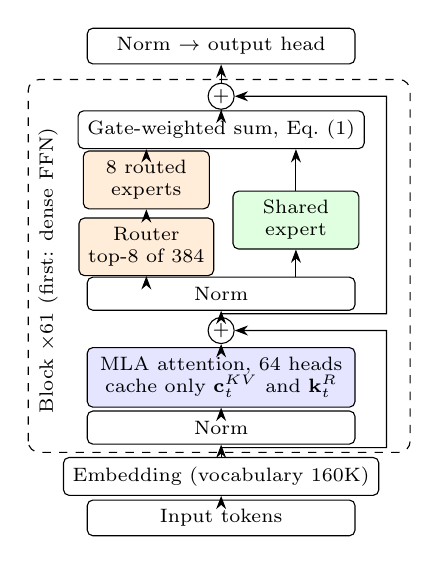
\begin{tikzpicture}[yscale=0.85, font=\scriptsize, >=Stealth,
  blk/.style={draw, rounded corners=2pt, minimum width=3.4cm, minimum height=0.42cm, align=center},
  sm/.style={draw, rounded corners=2pt, minimum width=1.6cm, minimum height=0.42cm, align=center}]
\node[blk] (in) at (0,0) {Input tokens};
\node[blk] (emb) at (0,0.62) {Embedding (vocabulary 160K)};
\node[blk] (n1) at (0,1.35) {Norm};
\node[blk, fill=blue!10] (mla) at (0,2.1) {MLA attention, 64 heads\\cache only $\mathbf{c}^{KV}_t$ and $\mathbf{k}^{R}_t$};
\node[draw, circle, inner sep=0.5pt] (p1) at (0,2.8) {$+$};
\node[blk] (n2) at (0,3.35) {Norm};
\node[sm, fill=orange!15] (rt) at (-0.95,4.05) {Router\\top-8 of 384};
\node[sm, fill=orange!15] (re) at (-0.95,5.05) {8 routed\\experts};
\node[sm, fill=green!12] (se) at (0.95,4.45) {Shared\\expert};
\node[blk] (sum) at (0,5.8) {Gate-weighted sum, Eq.~(1)};
\node[draw, circle, inner sep=0.5pt] (p2) at (0,6.3) {$+$};
\node[blk] (out) at (0,7.05) {Norm $\rightarrow$ output head};
\draw[->] (in) -- (emb);
\draw[->] (emb) -- (n1);
\draw[->] (n1) -- (mla);
\draw[->] (mla) -- (p1);
\draw[->] (p1) -- (n2);
\draw[->] (n2.north -| rt.south) -- (rt.south);
\draw[->] (n2.north -| se.south) -- (se.south);
\draw[->] (rt) -- (re);
\draw[->] (re.north) -- (re.north |- sum.south);
\draw[->] (se.north) -- (se.north |- sum.south);
\draw[->] (sum) -- (p2);
\draw[->] (p2) -- (out);
\draw[->] (0,1.05) -- (2.1,1.05) -- (2.1,2.8) -- (p1.east);
\draw[->] (0,3.05) -- (2.1,3.05) -- (2.1,6.3) -- (p2.east);
\draw[dashed, rounded corners] (-2.45,0.98) rectangle (2.4,6.55);
\node[rotate=90] at (-2.2,3.7) {Block $\times61$ (first: dense FFN)};
\end{tikzpicture}
\caption{Simplified Kimi K2 block, based on~\cite{kimik2,kimik2github,deepseekv3}. MLA compresses keys and values into a small cached latent vector. The router sends each token to 8 of 384 routed experts, and the shared expert processes every token.}
\label{fig:arch}
\end{figure}

\section{Attention Mechanism}
Standard multi-head attention (MHA) caches a key and a value per head for every previous token, so this key-value (KV) cache dominates memory in long generation. K2 uses Multi-head Latent Attention (MLA), introduced in DeepSeek-V2~\cite{deepseekv2} and used in DeepSeek-V3~\cite{deepseekv3,kimik2}. MLA compresses keys and values jointly into a low-rank latent vector:
\begin{align}
\mathbf{c}^{KV}_t&=W^{DKV}\mathbf{h}_t,\\
\mathbf{k}^{C}_t&=W^{UK}\mathbf{c}^{KV}_t,\qquad \mathbf{v}^{C}_t=W^{UV}\mathbf{c}^{KV}_t,\\
\mathbf{k}^{R}_t&=\mathrm{RoPE}\!\left(W^{KR}\mathbf{h}_t\right),
\end{align}
where $W^{DKV}$ is a down-projection and $W^{UK},W^{UV}$ are up-projections. Because rotary position embedding (RoPE) cannot be absorbed into the compressed path, a small decoupled key $\mathbf{k}^{R}_t$ carries the position information. During generation, only $\mathbf{c}^{KV}_t$ and $\mathbf{k}^{R}_t$ are cached~\cite{deepseekv3}. The cache per token per layer is therefore $d_c+d_h^R$ elements instead of $2n_hd_h$ for MHA~\cite{deepseekv2}. With the DeepSeek-V3 dimensions ($d_c=512$, $d_h^R=64$, $d_h=128$, $n_h=128$)~\cite{deepseekv3}, this is 576 elements instead of 32{,}768, about $57\times$ smaller. DeepSeek-V2 reports a 93.3\% smaller KV cache than its dense predecessor~\cite{deepseekv2}.

\textbf{Head count.} K2 uses 64 attention heads, whereas DeepSeek-V3 uses 128~\cite{kimik2}. In the team's experiments, doubling the heads improved validation loss by only 0.5--1.2\%, but at a sequence length of 128K it increased inference FLOPs by 83\%~\cite{kimik2}. Since agentic workloads involve long contexts, the team chose 64 heads.

\textbf{Long context.} Pre-training used a 4,096-token context. During annealing, the model was trained on 400B tokens at 4K length and then on 60B tokens at 32K length. The window was finally extended to 128K tokens with YaRN~\cite{kimik2,yarn}, which rescales the rotary frequencies. The later 0905 and Thinking releases support 256K tokens~\cite{kimik2thinking}.

\section{Training Methodology}
\textbf{MuonClip optimizer.} K2 is trained with Muon, which updates each weight matrix with an orthogonalized momentum computed by Newton--Schulz iterations. It achieves about $2\times$ the compute efficiency of AdamW~\cite{muon}. For a weight $W\in\mathbb{R}^{n\times m}$, one step is
\begin{align}
M_t&=\mu M_{t-1}+G_t,\qquad O_t=\mathrm{NS}(M_t)\cdot0.2\sqrt{\max(n,m)},\\
W_t&=W_{t-1}-\eta\left(O_t+\lambda W_{t-1}\right),
\end{align}
where the factor $0.2\sqrt{\max(n,m)}$ matches the update scale of AdamW and $\lambda$ is weight decay~\cite{kimik2,muon}. At scale, however, Muon caused attention logits to explode: in a mid-scale run they quickly exceeded 1000~\cite{kimik2}. QK-Clip fixes this by rescaling the query and key projections of each head after an update. For head $h$, it computes the maximum logit over the batch $B$:
\begin{align}
S^{h}_{\max}&=\frac{1}{\sqrt{d}}\max_{X\in B}\max_{i,j}\mathbf{Q}^{h}_i\mathbf{K}^{h\top}_j,\\
\gamma_h&=\min\!\left(1,\tau/S^{h}_{\max}\right).
\end{align}
For MLA, the head-specific query and key components $W^h_{qc}$ and $W^h_{kc}$ are each multiplied by $\sqrt{\gamma_h}$, and the rotary query $W^h_{qr}$ by $\gamma_h$. The shared rotary key is not changed, because it affects all heads~\cite{kimik2}. With $\tau=100$, the logits rose to the cap and then decayed to a stable range after about 30\% of training, so the clip turns itself off. Training was completed on 15.5T tokens without a single loss spike~\cite{kimik2}.

\textbf{Data and schedule.} The corpus covers four domains: web text, code, mathematics, and knowledge. To use high-quality tokens more efficiently, knowledge texts are rephrased in different styles and math texts are rewritten as learning notes~\cite{kimik2}. In an ablation, ten rephrasings with one epoch raised SimpleQA accuracy from 23.76 (raw text, ten epochs) to 28.94~\cite{kimik2}. Training used a warmup--stable--decay schedule: 10T tokens at a learning rate of $2\times10^{-4}$, then 5.5T tokens with cosine decay to $2\times10^{-5}$, with weight decay 0.1 and a global batch of 67M tokens~\cite{kimik2}.

\textbf{Infrastructure.} Training ran on NVIDIA H800 clusters. Each node has 8 GPUs, 2 TB of RAM, and $8\times400$\,Gbps RoCE links~\cite{kimik2}. The model combines 16-way pipeline parallelism with virtual stages, 16-way expert parallelism, and ZeRO-1 data parallelism, and it can train on any multiple of 32 nodes. To fit about 30\,GB of states per GPU, activations are reduced with selective recomputation, FP8 storage of insensitive activations, and CPU offloading~\cite{kimik2}.

\textbf{Post-training and RL.} Supervised fine-tuning also uses Muon. Its agentic data are synthesized with more than 3,000 real MCP tools and over 20,000 synthetic tools, simulated users and environments, and rubric-based LLM judges~\cite{kimik2}. RL then combines verifiable rewards with a self-critique rubric reward. Verifiable rewards cover mathematics, instruction following, faithfulness, coding in more than 10,000 concurrent sandboxes, and safety. For open-ended tasks, the model acts as its own rubric-based critic. The algorithm adds per-task token budgets, a PTX loss on curated data, and temperature decay~\cite{kimik2}.

\section{Inference and Performance}
\textbf{Compute and complexity.} Per token, the FFN cost scales with the nine active experts rather than the 385 stored experts. Each token thus costs roughly as much as in a 32B dense model, about $2\times32$B $\approx64$ GFLOPs per forward pass by the common $2N$ estimate. Attention cost grows linearly with context length per generated token, and quadratically over a full sequence, in proportion to the number of heads. Halving the heads therefore saves most at long contexts~\cite{kimik2}.

\textbf{Memory and scalability.} Sparse activation does not reduce memory: all 1.04T parameters must be stored, because any expert may be selected. The checkpoints are published in block-FP8 format~\cite{kimik2github}, which at one byte per parameter needs about 1\,TB for the weights alone, so serving requires multi-GPU nodes with expert parallelism. The recommended engines are vLLM, SGLang, KTransformers, and TensorRT-LLM~\cite{kimik2github}. Kimi K2 Thinking applies INT4 weight-only quantization to the MoE components and reports about $2\times$ faster generation~\cite{kimik2thinking}.

\textbf{Benchmarks.} Table~\ref{tab:bench} compares Kimi-K2-Instruct with two open MoE baselines~\cite{kimik2}. K2 leads on agentic coding, scoring 65.8 on SWE-bench Verified compared with 38.8 for DeepSeek-V3-0324. It also leads on tool use ($\tau^2$-Bench) and competitive coding (LiveCodeBench v6), while remaining strong on mathematics and general knowledge.

\begin{table}[t]
\centering
\caption{Architecture of Kimi K2 and DeepSeek-V3~\cite{kimik2,kimik2github,deepseekv3}}
\label{tab:spec}
\begin{tabular}{lcc}
\toprule
 & DeepSeek-V3 & Kimi K2 \\
\midrule
Total / activated parameters & 671B / 37B & 1.04T / 32.6B \\
Layers (dense layers) & 61 (3) & 61 (1) \\
Hidden / expert dimension & 7168 / 2048 & 7168 / 2048 \\
Routed + shared experts (active) & 256+1 (8+1) & 384+1 (8+1) \\
Expert grouping & Yes & No \\
Attention (heads) & MLA (128) & MLA (64) \\
Pre-training tokens & 14.8T & 15.5T \\
Optimizer & AdamW & MuonClip \\
\bottomrule
\end{tabular}
\end{table}

\begin{table}[t]
\centering
\caption{Selected results of instruct models in non-thinking mode, from~\cite[Table~3]{kimik2}}
\label{tab:bench}
\setlength{\tabcolsep}{4pt}
\begin{tabular}{lccc}
\toprule
Benchmark (metric) & K2 & DS-V3$^{a}$ & Qwen3$^{b}$ \\
\midrule
SWE-bench Verified (Pass@1)$^{c}$ & \textbf{65.8} & 38.8 & 34.4 \\
LiveCodeBench v6 (Pass@1) & \textbf{53.7} & 46.9 & 37.0 \\
$\tau^2$-Bench retail (Avg@4) & \textbf{70.6} & 69.1 & 57.0 \\
$\tau^2$-Bench airline (Avg@4) & \textbf{56.5} & 39.0 & 26.5 \\
ACEBench (Acc.) & \textbf{76.5} & 72.7 & 70.5 \\
AIME 2025 (Avg@64) & \textbf{49.5} & 46.7 & 24.7$^{*}$ \\
GPQA-Diamond (Avg@8) & \textbf{75.1} & 68.4$^{*}$ & 62.9$^{*}$ \\
MMLU-Redux (EM) & \textbf{92.7} & 90.5 & 89.2$^{*}$ \\
\bottomrule
\multicolumn{4}{p{0.95\columnwidth}}{\footnotesize $^{a}$DeepSeek-V3-0324. $^{b}$Qwen3-235B-A22B. $^{c}$Agentic, single attempt. $^{*}$Taken by~\cite{kimik2} from the model's own report or blog.}
\end{tabular}
\end{table}

\section{Architectural Innovations}
Kimi K2 introduces no new layer type: it reuses the DeepSeek-V3 blocks (MLA, shared-plus-routed experts, sigmoid gating)~\cite{deepseekv3} but differs in five ways:
\begin{enumerate}
\item \emph{Higher sparsity:} 384 experts with sparsity 48 instead of 256 and 32, chosen by a sparsity scaling law; total parameters grow by 54\% while activated ones fall by 13\%~\cite{kimik2}. Unlike classic sparse MoE~\cite{shazeer2017}, it pairs fine-grained experts with a shared expert.
\item \emph{Cheaper attention:} 64 instead of 128 heads, which trades a small loss improvement for 83\% fewer long-context inference FLOPs~\cite{kimik2}.
\item \emph{Simpler routing:} no expert grouping and only one dense layer~\cite{kimik2}.
\item \emph{MuonClip:} per-head QK-Clip makes Muon training stable at trillion scale, without loss spikes~\cite{kimik2}.
\item \emph{Agentic post-training:} large-scale tool-use data synthesis and RL with self-critique rubric rewards~\cite{kimik2}.
\end{enumerate}

\section{Conclusion}
Kimi K2 refines an existing MoE design rather than replacing it. Its 1.04T-parameter, 32B-active architecture combines very sparse expert routing with MLA and a reduced head count, so that long-context agentic inference stays affordable. MuonClip stabilized training over 15.5T tokens, and agentic data and RL made it a strong tool-using agent. The main remaining cost is memory, since all experts must be stored. The report also notes that the model can produce excessive tokens on hard reasoning tasks~\cite{kimik2}.

\bibliographystyle{IEEEtran}
\bibliography{references}

\end{document}
